\chapter{Sobre la complejidad de H y el ruido}

En este capítulo, trataremos la dificultad que introduce la aparición de
ruido en las etiquetas a la hora de elegir la clase de funciones más adecuadas.

\section{Dibujar gráficas de nubes de puntos simuladas}

\subsection{Uniformemente distribuidos}

\textbf{Considere $N = 50$, $\dim = 2$, $rango = [-50, 50]$ con
\mintinline{python}{simula_unif(N, dim, rango)}}

\begin{figure}[H]
\centering
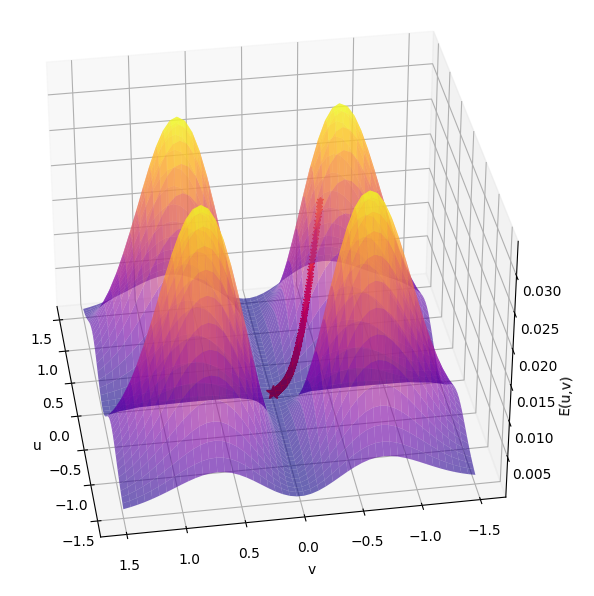
\includegraphics[width=0.6\textwidth]{Figure_1.png}
\caption{Gráfica de nube de puntos uniformemente distribuidos}
\end{figure}

\subsection{Siguiendo distribución gaussiana de media \texorpdfstring{$0$} y varianza dada}

\textbf{Considere $N = 50$, $dim = 2$ y $sigma = [5, 7]$ con 
\mintinline{python}{simula_gauss(N, dim, sigma)}}

\begin{figure}[H]
\centering
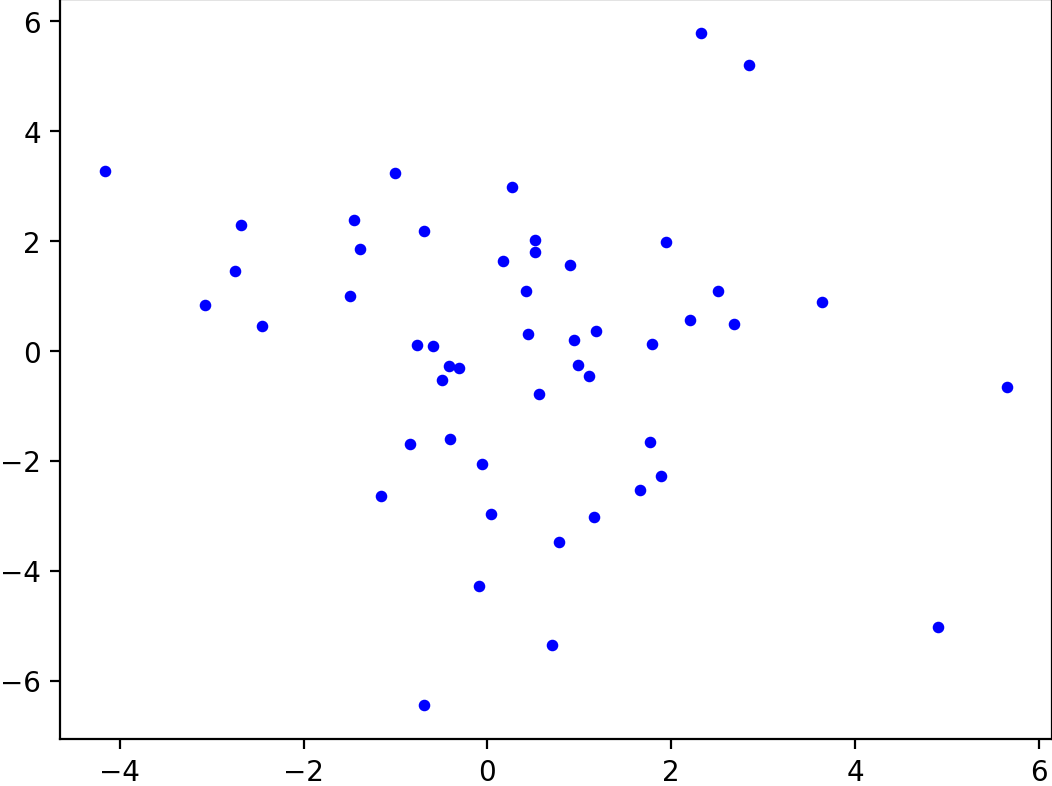
\includegraphics[width=0.6\textwidth]{Figure_2.png}
\caption{Gráfica de nube de puntos en distribución gaussiana.}
\end{figure}

\section{Ejercicio 2}

Vamos a valorar la influencia del ruido en la selección de la complejidad de la
clase de funciones.  Con ayuda de la función
\mintinline{python}{simula_unif(100, 2, [-50, 50])} generamos una muestra de
puntos 2D a los que vamos añadir una etiqueta usando el signo de la función 
$f(x, y) = y - ax - b$, es decir el signo de cada punto con respecto a la
recta simulada con \mintinline{python}{simula_recta()}.  

\subsection{Dibujo de puntos con etiqueta y recta usada}

Dibujamos un gráfico 2D con los puntos clasificados por etiquetas junto
con la recta usada para etiquetar. 

\begin{figure}[H]
\centering
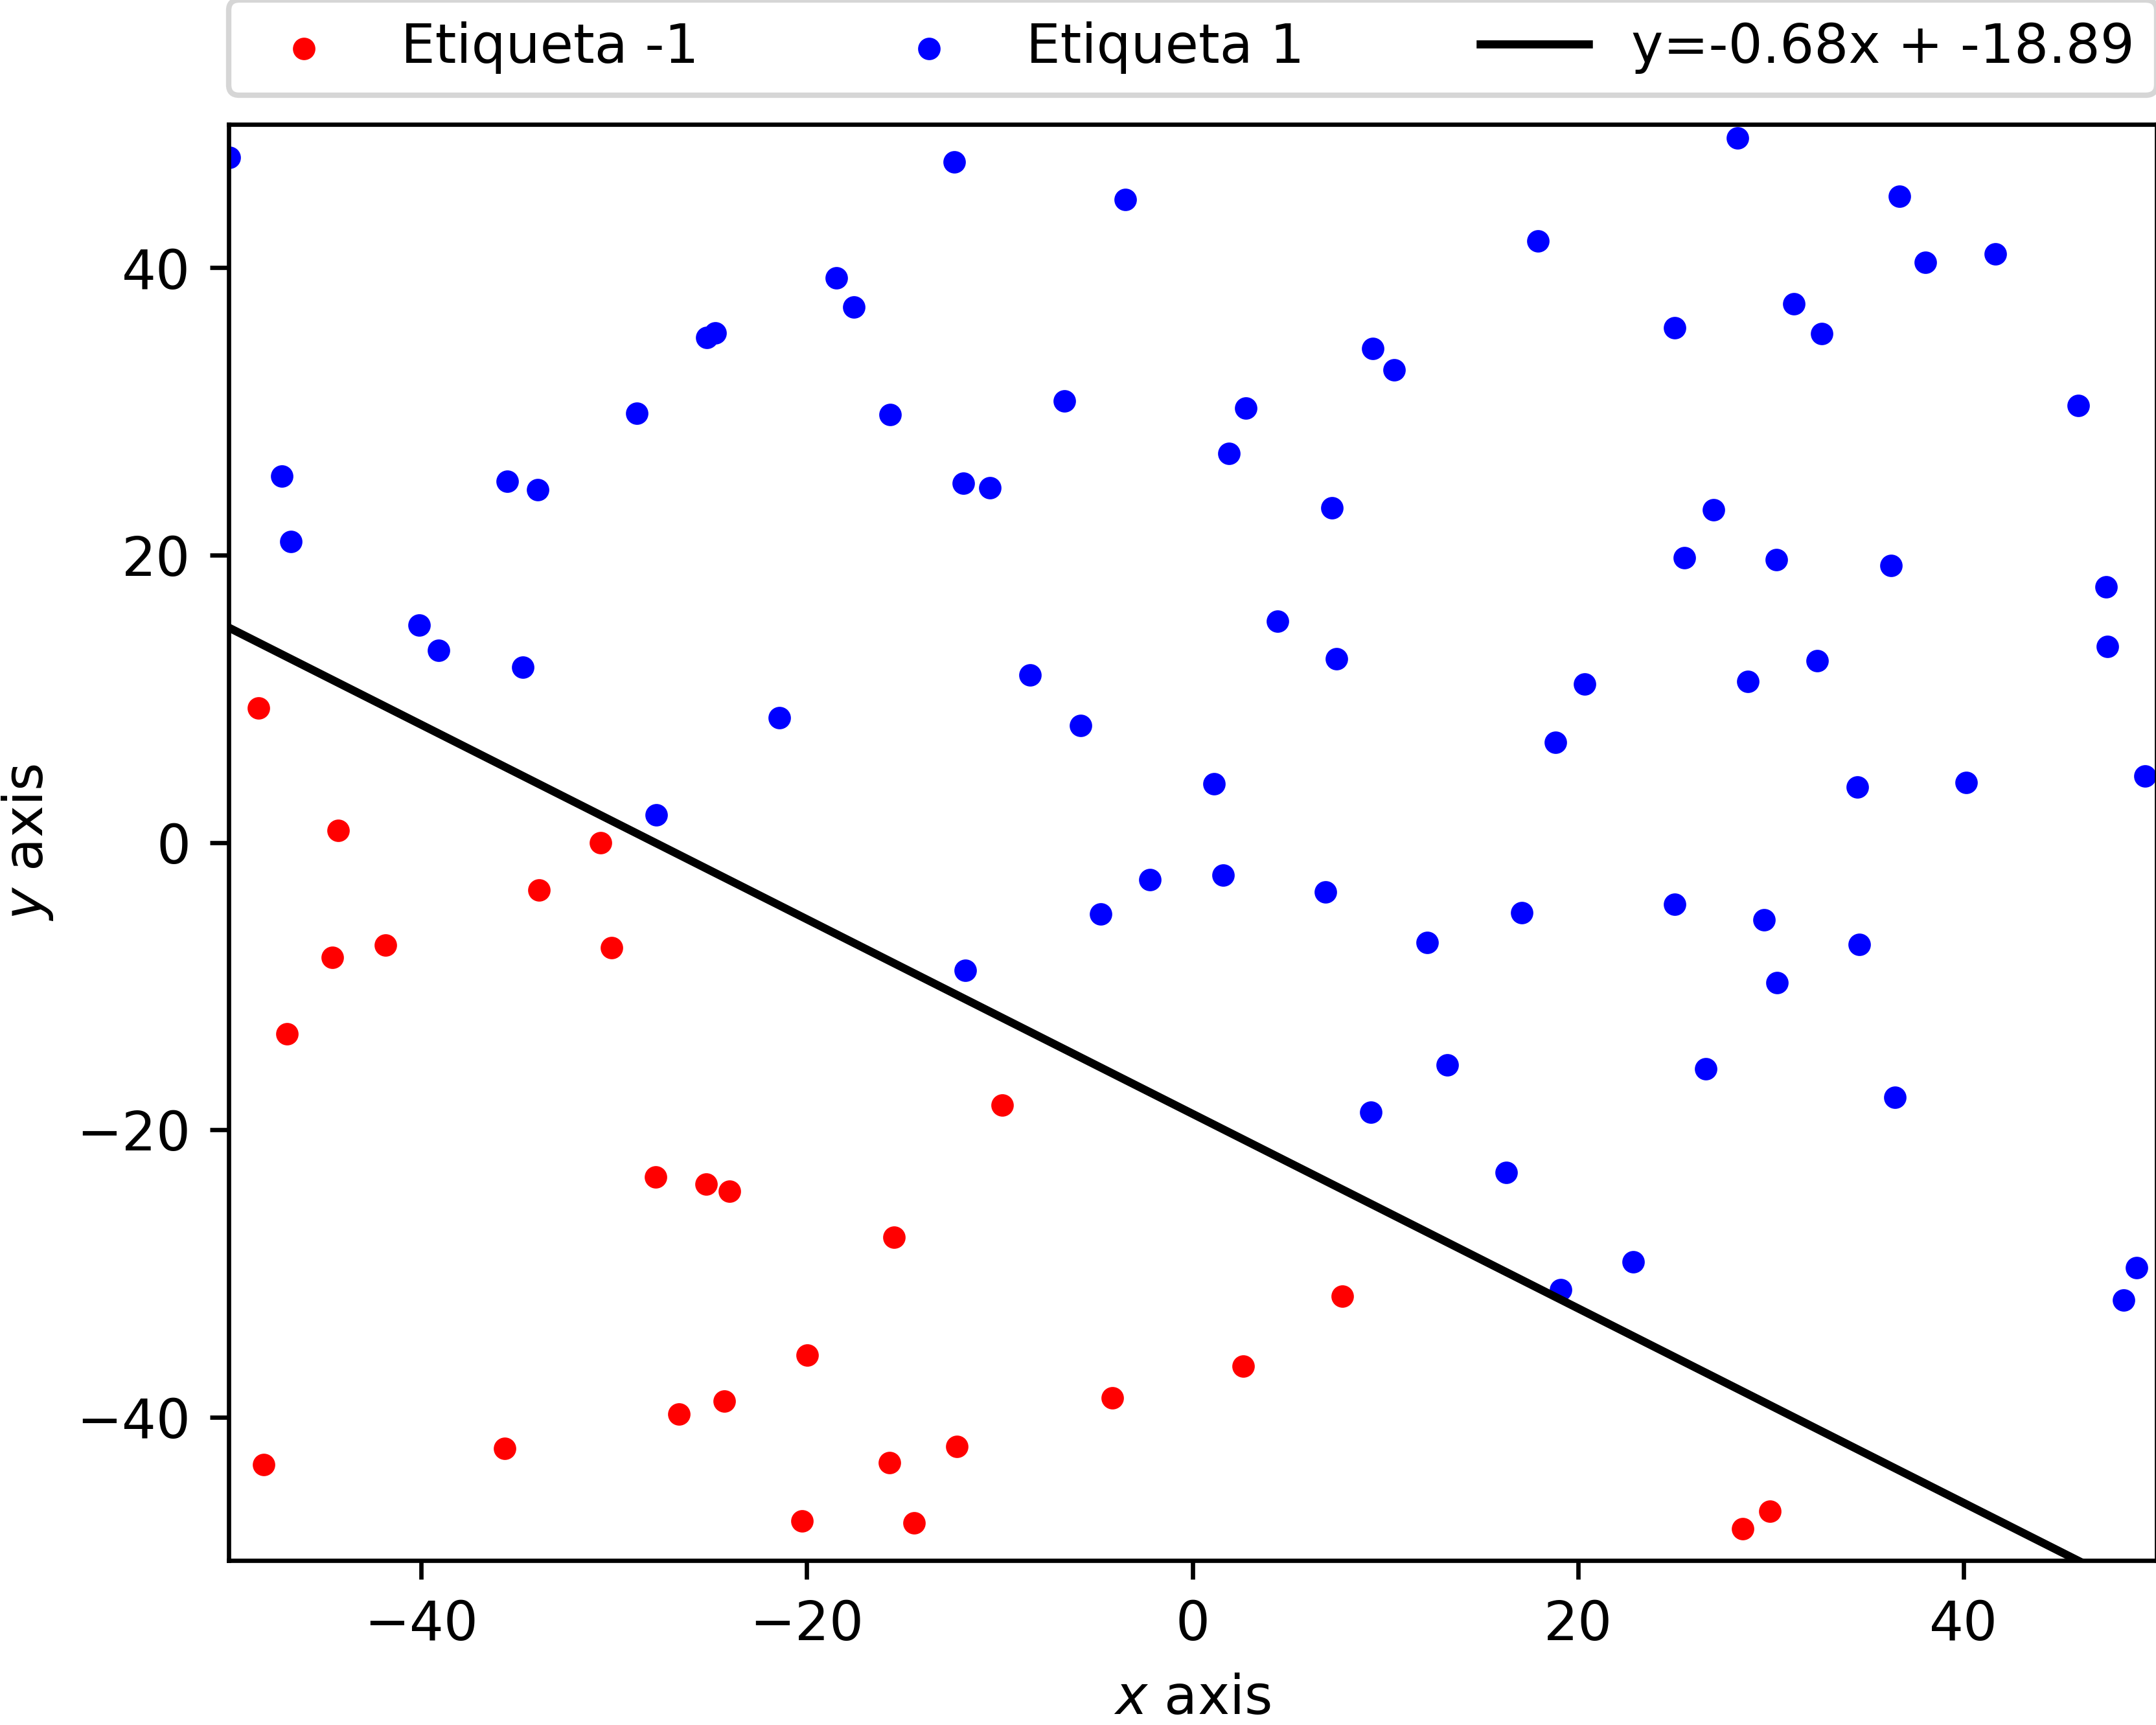
\includegraphics[width=0.6\textwidth]{Figure_3.png}
\caption{Etiquetado de puntos uniformemente distribuidos según recta.}
\end{figure}

Es claro que si usamos una recta para clasificar los puntos en dos etiquetas,
estos datos está bien clasificados por esta recta.

\subsection{Añadir ruido aleatorio}

Modifique de forma aleatoria un $10\%$ de las etiquetas positivas y otro $10\%$
de las negativas y guarde los puntos con sus nuevas etiquetas. Dibuje de nuevo
la gráfica anterior. Ahora habrá puntos mal clasificados respecto de la recta.  

\begin{figure}[H]
\centering
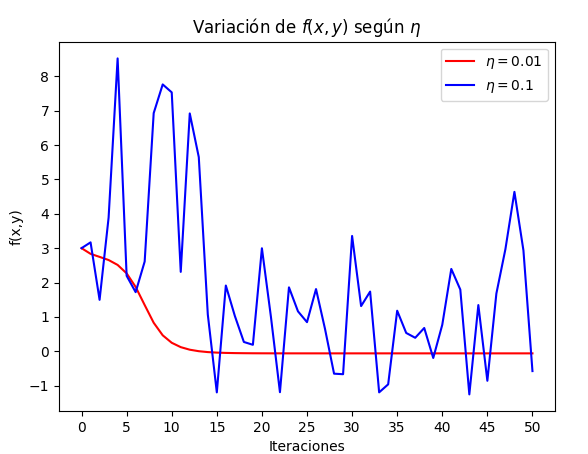
\includegraphics[width=0.6\textwidth]{Figure_4.png}
\caption{Nube de puntos anterior con 10\% de ruido en cada etiqueta.}
\end{figure}

En efecto, $3$ puntos con etiqueta $-1$ (rojos) ahora tienen etiqueta $1$
(son azules). Esto es el $10\%$ del total ($27$) redondeado.

\subsection{Otras fronteras de clasificación}

Supongamos ahora que las siguientes funciones definen la frontera de
clasificación de los puntos de la muestra en lugar de una recta 

\begin{itemize}
\item $f(x,y) = (x - 10)^2 + (y - 20)^2 - 400$
\item $f(x,y) = 0.5(x + 10)^2 + (y - 20)^2 - 400$
\item $f(x,y) = 0.5(x - 10)^2 - (y + 20)^2 - 400$
\item $f(x,y) = y - 20x^2 - 5x + 3$
\end{itemize}

Visualizar el etiquetado generado en el apartado 2b junto con la gráfica de cada
una de las funciones.  Comparar las regiones positivas y negativas de estas
nuevas funciones con las obtenidas en el caso de la recta.  Argumente si estas
funciones más complejas son mejores clasificadores que la función lineal.
Observe las gráficas y diga qué consecuencias extrae sobre la influencia de la
modificación de etiquetas en el proceso de aprendizaje. Explique el
razonamiento. 